\documentclass[12pt]{article}
\usepackage[paperwidth=13.333in,paperheight=7.5in,margin=0.55in]{geometry}
\usepackage{times,xcolor,graphicx,booktabs,tikz,hyperref,fancyhdr}
\usetikzlibrary{positioning}
\definecolor{maroon}{HTML}{500000}
\definecolor{cream}{HTML}{FFF8E7}
\definecolor{gold}{HTML}{C9A24B}
\definecolor{muted}{HTML}{5D554C}
\setlength{\parindent}{0pt}
\pagestyle{fancy}
\fancyhf{}
\cfoot{\footnotesize\color{muted}\thepage\,/\,10}
\renewcommand{\headrulewidth}{0pt}
\hypersetup{colorlinks=true,urlcolor=maroon}
\newcommand{\slidehead}[1]{{\color{maroon}\rule{\linewidth}{4pt}}\par\vspace{2pt}{\LARGE\bfseries\color{maroon}#1}\par\vspace{4pt}}
\newcommand{\notes}[1]{\vfill{\color{gold}\rule{\linewidth}{1pt}}\\[2pt]{\fontsize{8.5}{10}\selectfont\color{muted}\textbf{Speaker notes.} #1}}
\begin{document}

% 1
\begin{center}
\vspace{1.1in}
{\color{maroon}\rule{0.8\linewidth}{6pt}}\\[12pt]
{\Huge\bfseries\color{maroon} Aggie Course Scout}\\[8pt]
{\Large A fielded BM25F search engine over the public TAMU course catalog}\\[18pt]
{\large Carlos Luna-Pena \quad CSCE 470 \quad Fall 2026}\\[4pt]
{\large \url{https://clmoon2.github.io/aggie-course-scout/}}
\end{center}
\notes{Hi. This is Aggie Course Scout, a search engine over the official TAMU catalog. I built it solo. It's static, public-data only, and the whole thing is on GitHub Pages. I'll show the data, the ranking, the deployed UI, and the corrected evaluation. It's a class project, not an official TAMU tool, and the data is public. The repo has the crawler, the index builder, and every judgment so you can rerun it. The measured latency and the exact test commands are in the handoff.}
\newpage

% 2
\slidehead{The lookup problem}
\begin{minipage}[t]{0.58\linewidth}
The catalog has descriptions. It doesn't have a course search.
\vspace{6pt}
\begin{itemize}
  \item Searching \texttt{security} on the catalog can return a policy page before CSCE 465.
  \item A student who remembers ``that networks class'' gets a department list and browser find.
  \item Advisors do the same lookup by hand.
  \item The schedule answers \emph{when} a section meets. It doesn't answer \emph{what the course covers}.
\end{itemize}
\vspace{4pt}
The job is narrow: find a course by topic, show the official text, explain the rank.
\end{minipage}\hfill
\begin{minipage}[t]{0.38\linewidth}
\colorbox{cream}{\parbox{0.92\linewidth}{\vspace{4pt}\textbf{Who benefits}\\[3pt]Students planning a term. Advisors doing a fast lookup. Anyone building a degree plan who needs the description.\vspace{4pt}}}
\end{minipage}
\notes{The catalog search is site search, not course search. That distinction is the whole motivation. I'm not replacing the schedule or the audit. Every record links back to the official page. Search should answer topic first and link out for logistics. The form keeps a visible syntax line instead of hiding filters in a menu. The empty state explains what to try instead of just saying zero.}
\newpage

% 3
\slidehead{Data, and what it cost}
\begin{minipage}[t]{0.52\linewidth}
\begin{tabular}{@{}lr@{}}
\toprule
Department pages & 383\\
HTTP 200 & 383\\
HTTP 404 & 0\\
Empty pages & 7\\
Unique records & 10,277\\
Undergrad / grad & 5,262 / 5,015\\
Other/Professional & 36\\
Prereq lines parsed & 8,564\\
\bottomrule
\end{tabular}
\vspace{5pt}

Crawler: requests + BeautifulSoup, 4 workers, 0.2 s delay, 3 retries, robots.txt checked, raw pages gzipped. Four-digit codes were added after the first pass and brought back DDHS and LAW.
\end{minipage}\hfill
\begin{minipage}[t]{0.44\linewidth}
\textbf{Fields.} code, title, credits, description, prerequisites, department, college, level, URL.
\vspace{5pt}

\textbf{Cleaning.} strip HTML, collapse spaces, remove hour boilerplate, split prereqs, dedupe level plus code, hash the output.
\vspace{5pt}

\textbf{Caveats.} College is hand-mapped because it isn't on the page. The count is above my proposed range because research and seminar records are real courses.
\end{minipage}
\notes{No 404s. Seven department pages have zero course blocks, so they contribute no records. The count came in high, and I kept it rather than trimming real courses. That distinction got lost in an earlier slide and is fixed. Eight records also have empty descriptions and are kept, which the report discloses. The crawl manifest records bytes and a SHA for every page.}
\newpage

% 4
\slidehead{BM25F, four fields}
\begin{minipage}[t]{0.56\linewidth}
\[
\mathrm{score}(q,d)=\sum_{t\in q}\mathrm{idf}(t)\frac{S_{t,d}(k_1+1)}{k_1+S_{t,d}}
\]
\[
S_{t,d}=\sum_f w_f\frac{\mathrm{tf}_{t,d,f}}{1-b+b|d_f|/\mathrm{avg}_f}
\]
\[
\mathrm{idf}(t)=\ln\left(1+\frac{N-\mathrm{df}(t)+0.5}{\mathrm{df}(t)+0.5}\right)
\]
\(k_1=1.2\), \(b=0.75\).
\end{minipage}\hfill
\begin{minipage}[t]{0.40\linewidth}
\begin{tabular}{@{}lr@{}}
\toprule
Field & Weight\\
\midrule
Title & 3.0\\
Department & 2.0\\
Description & 1.0\\
Prerequisite & 0.5\\
\bottomrule
\end{tabular}
\vspace{8pt}

Quoted phrases get a bonus, doubled in the title. Filters apply after scoring. The same formula runs in Python and the browser.
\end{minipage}
\notes{This is standard BM25F. Weighted term frequencies are summed per field and saturated once. The formula has one saturation per term, not per field. That's deliberate: it keeps title and description evidence comparable. Same corpus in, same artifact out. The gzip mtime is zero and terms are sorted, which removes the old nondeterministic hash. The 401,031 postings are all checked against document lengths in a test.}
\newpage

% 5
\slidehead{Query layer}
\begin{minipage}[t]{0.47\linewidth}
\textbf{Parsing}
\begin{itemize}
  \item quoted phrases, including one word
  \item \texttt{dept:csce}, \texttt{college:college-of-engineering}, \texttt{credits:1-2}
  \item repeated credit bounds, \texttt{-term} from all fields
  \item synonyms: ml, ai, db, os, security, stats
  \item Damerau-Levenshtein suggestion, one edit short, two long
\end{itemize}
\end{minipage}\hfill
\begin{minipage}[t]{0.49\linewidth}
\textbf{Presentation}
\begin{itemize}
  \item facets from the filtered set
  \item highlighted snippets
  \item why panel: term, field, TF, weighted TF, term score
  \item loading, empty, error, retry states
\end{itemize}
\vspace{4pt}
\colorbox{cream}{\parbox{0.9\linewidth}{\vspace{3pt}The Python evaluator and the JavaScript engine share the same terms and tie-break. If the browser drifts from the evaluator, the test fails. Negation now unions all four posting fields, not just descriptions. Quoted one-word phrases now score instead of returning zero.\vspace{3pt}}}
\end{minipage}
\notes{The parser fixes matter. Earlier, \texttt{-csce} only removed description matches, a quoted single word returned zero, and two credit filters overwrote each other. College facet values are slugs so names with spaces stay one token. The same stemmer and tokenizer run in both languages, and the parity test compares top-ten ids on all 25 queries.}
\newpage

% 6
\slidehead{What it looks like}
\begin{minipage}[t]{0.54\linewidth}
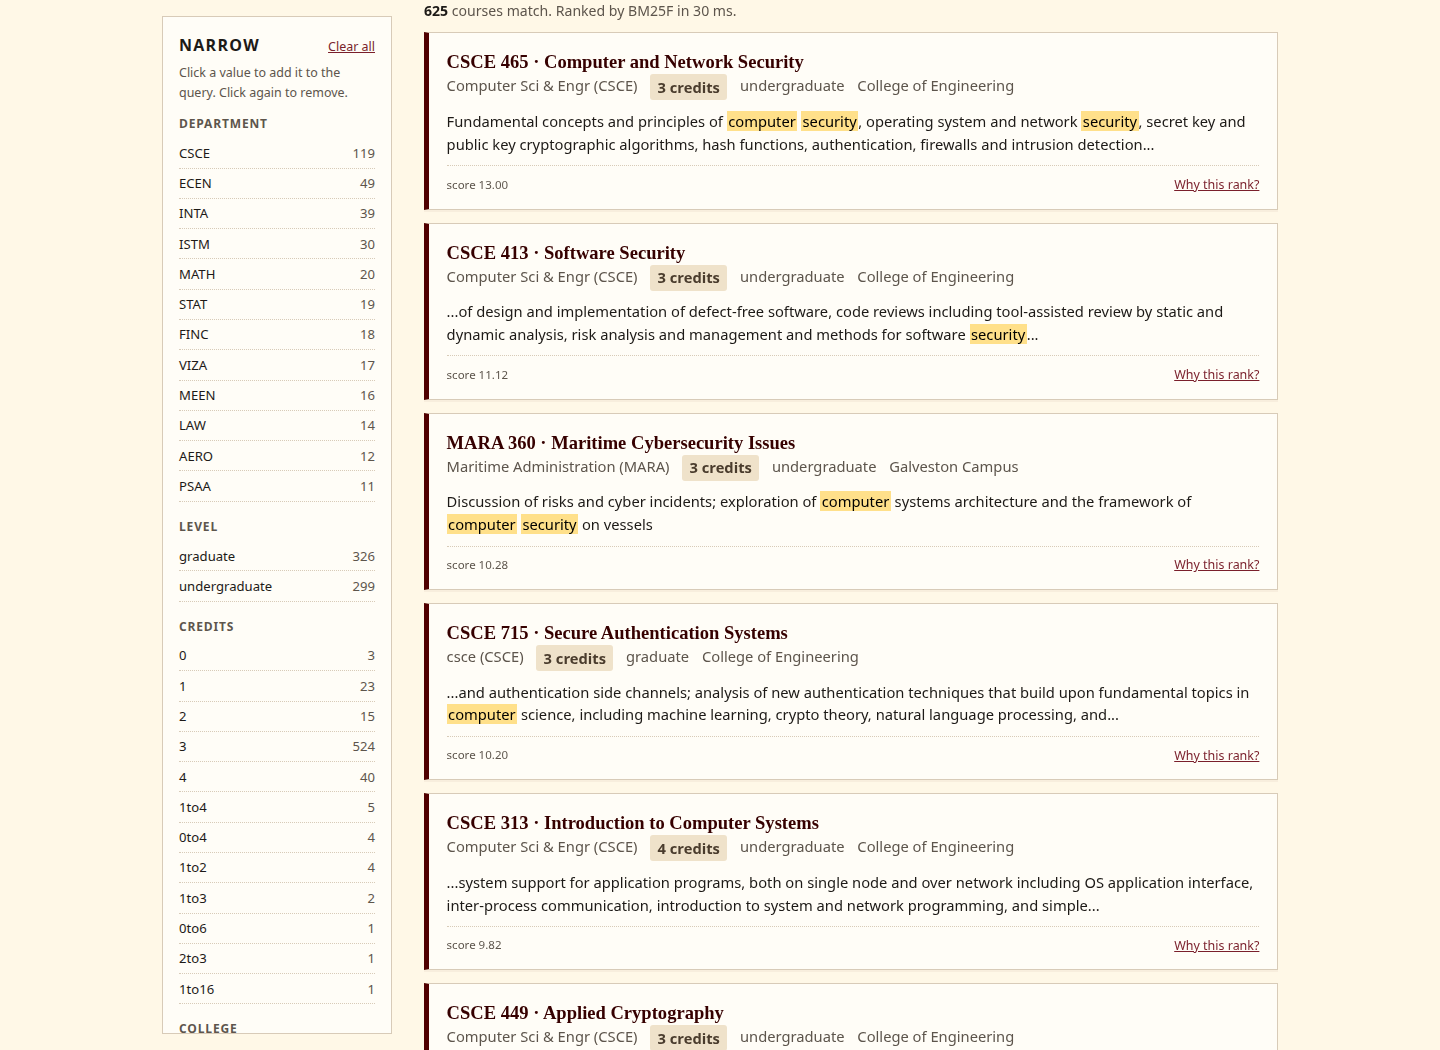
\includegraphics[height=4.3in,keepaspectratio]{../web/assets/screenshots/desktop-results.png}
\end{minipage}\hfill
\begin{minipage}[t]{0.43\linewidth}
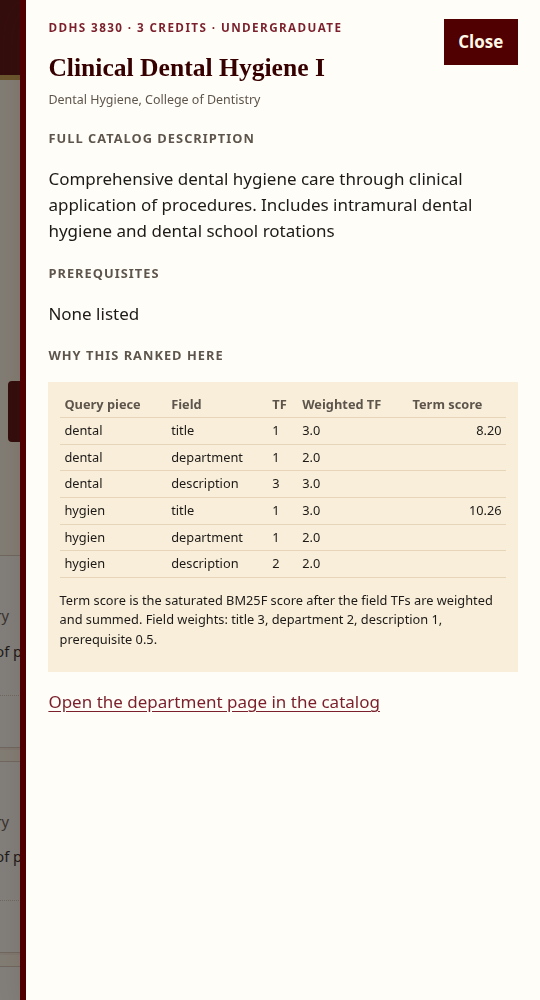
\includegraphics[height=4.3in,keepaspectratio]{../web/assets/screenshots/detail-drawer.png}
\vspace{4pt}

{\footnotesize Left: filtered facets, marked snippets, score, and a why-this-rank control on every card. Right: detail drawer with prerequisites and the term-by-term score table over a backdrop.}\vspace{4pt}

\colorbox{cream}{\parbox{0.95\linewidth}{\vspace{3pt}\small The why table is the ranking evidence: field, TF, weighted TF, and the term score. Facet counts come from the filtered set, not the whole index.\vspace{3pt}}}
\end{minipage}
\notes{This is the actual product, not a mock. The College of Dentistry facet advertises 159 and returns 159. Credit buckets match their counts. The drawer traps focus, restores it on close, and the backdrop closes it. The page auto-scrolls to the summary on a phone, and the detail sheet is a real modal with Escape and backdrop close. The mobile jump and focus restore are covered too. The facet buttons expose pressed state and selected styling. The detail view no longer prints the snippet twice.}
\newpage

% 7
\slidehead{How I tested it}
\begin{minipage}[t]{0.50\linewidth}
\begin{itemize}
  \item 25 queries: 7 short known-item, 7 exploratory, 5 typo, 6 synonym
  \item same correction and synonyms for baselines and BM25F
  \item top 10 pooled from 2 baselines and 7 BM25F conditions
  \item 514 pairs, rule-labeled 0/1/2, 4 manual overrides
  \item global NDCG ideal from the full judged pool
  \item 5,000-resample paired bootstrap and exact sign test
\end{itemize}
\end{minipage}\hfill
\begin{minipage}[t]{0.46\linewidth}
\textbf{Grading rule}\par\vspace{2pt}
\begin{tabular}{@{}ll@{}}
\toprule
Grade & Rule\\
\midrule
2 & requested code or intent phrase in title\\
1 & intent phrase in description\\
0 & otherwise\\
\bottomrule
\end{tabular}
\vspace{8pt}

Latency: 75 in-page searches, headless Chromium, p50 and p95.
\vspace{10pt}

\colorbox{cream}{\parbox{0.94\linewidth}{\vspace{3pt}\small Why 25? Enough to cover four buckets and keep 514 judgments manageable for one grader. A second grader is the next step.\vspace{3pt}}}
\end{minipage}
\notes{One grader and 25 queries is small, and most labels come from a rule that reuses the query string. So this measures lexical title match more than topical relevance. The labels are rule-generated with four overrides, not human gold. The sign test is exact, so it doesn't assume normality. We kept the per-query deltas in the results folder for inspection. Four manual overrides are listed with notes.}
\newpage

% 8
\slidehead{Results}
\begin{minipage}[t]{0.55\linewidth}
\begin{tabular}{@{}lrrrr@{}}
\toprule
Condition & P@10 & NDCG@10 & AP@10 & MRR\\
\midrule
TF-IDF, same terms & 0.700 & 0.671 & 0.669 & 0.794\\
Flat BM25, same terms & 0.740 & 0.723 & 0.724 & 0.853\\
\textbf{BM25F} & \textbf{0.776} & \textbf{0.793} & \textbf{0.767} & \textbf{0.841}\\
No correction & 0.652 & 0.652 & 0.638 & 0.717\\
No synonyms & 0.720 & 0.734 & 0.708 & 0.798\\
No syn.\ or corr. & 0.596 & 0.593 & 0.580 & 0.673\\
Title only & 0.716 & 0.806 & 0.716 & 0.873\\
No dept & 0.748 & 0.771 & 0.727 & 0.842\\
Equal weights & 0.788 & 0.795 & 0.794 & 0.868\\
\bottomrule
\end{tabular}
\vspace{3pt}

{\scriptsize Deduped codes: BM25F 0.756 P@10 / 0.790 NDCG; flat 0.716 / 0.722.}
\end{minipage}\hfill
\begin{minipage}[t]{0.42\linewidth}
\textbf{BM25F minus flat}
\begin{tabular}{@{}lrr@{}}
\toprule
Metric & Mean & 95\% CI\\
\midrule
P@10 & +0.036 & -0.004 to 0.080\\
NDCG & +0.070 & 0.020 to 0.126\\
AP@10 & +0.042 & -0.018 to 0.112\\
MRR & -0.012 & -0.043 to 0.018\\
\bottomrule
\end{tabular}
\vspace{6pt}

Latency p50 12.0 ms, p95 24.2 ms.
\end{minipage}
\notes{BM25F is ahead on NDCG. The interval excludes zero, 17 queries win and 5 lose, sign test p equals 0.017. But P@10 and AP cross zero, and MRR is a small loss. Correction is worth 0.141 NDCG inside the system and synonyms 0.059, but the 0.070 gap is the ranking comparison with both features held constant. It answers whether duplicates drive the gap. The answer is no: the deduped gap is 0.068 NDCG, almost unchanged. MRR is the one metric where flat BM25 is ahead.}
\newpage

% 9
\slidehead{Where it breaks}
\begin{itemize}
  \item \textbf{operating vs operations.} Both stem to \texttt{oper}. For \texttt{os}, SCMT 661 Operations Strategy is rank 3.
  \item \textbf{software is a modifier.} CSCE 429 Software Development and CSCE 713 Software Security sit at ranks 4 and 5 for ``software engineering.''
  \item \textbf{sense collision.} ``security'' returns LAW 706 Securities Regulation first, and the rule grades it 0.
  \item \textbf{acronym blast.} \texttt{os} returns 1,908 records because the expansion splits into common terms.
  \item \textbf{label and duplicate limits.} The rule reuses query strings, and 96 cross-level pairs appear twice.
\end{itemize}
\vspace{4pt}
\colorbox{cream}{\parbox{0.94\linewidth}{\vspace{3pt}The 0.070 NDCG gap is field weighting with features held constant. The 0.141 correction effect is inside BM25F with features removed. They aren't pieces of each other.\vspace{3pt}}}
\notes{These are the failures I'd fix first. The stemming collision is easy to reproduce. The software example shows term independence. The LAW result shows the labeler and the ranker agree it's the wrong sense, but the stem can't tell. Both are in the limitations. The known-item label rule also gets a caveat because it reuses the query string. The acronym os still returns 1,908 records, which is too broad.}
\newpage

% 10
\slidehead{Takeaway}
\begin{minipage}[t]{0.62\linewidth}
BM25F is ahead on NDCG, ties on P@10 and AP, and loses MRR. The title-only variant beats it. That's narrower than my first draft claimed.
\vspace{8pt}

The useful part isn't the score. It's the inspectable pipeline: public crawl, hashed data, one index shared by the evaluator and the browser, paired intervals, and a why panel a person can argue with.
\vspace{8pt}

Next: title bigrams, dedupe cross-level codes, retune the weights, and get a second grader.
\end{minipage}\hfill
\begin{minipage}[t]{0.34\linewidth}
\textbf{Live}\\
\url{https://clmoon2.github.io/aggie-course-scout/}
\vspace{6pt}

\textbf{Code}\\
\url{https://github.com/clmoon2/aggie-course-scout}
\vspace{6pt}

\textbf{Report}\\
\url{https://clmoon2.github.io/aggie-course-scout/report.html}
\end{minipage}
\notes{So the honest takeaway is narrow. The weights help NDCG on a small set, most of the product value is correction and filters, and the other metrics won't back a stronger claim. The corrected report is linked here. I'd rather defend the narrow version than the first draft. If you take one thing, take the correction method.}

\end{document}
